% Drawing 144/09-4 -- folder 144, batch 09, archive page 167 (PDF page 168).
% Transcription: $\sigma^2$ — un cercle traversé par deux diamètres perpendiculaires ; plus bas, un hexagone dont les côtés ne se rejoignent pas, et un cercle portant les points $a_1, c_0, b_0, a_0, c_3, b_3, a_3, c_2, b_2, a_2, c_1, b_1$, traversé de deux droites pleines et de segments en pointillés.
% Kind: circle with two diameters; broken hexagon; circle with twelve points. Method 2 (schematic redraw from the facsimile). Status: ok.
% Notes: Under sigma^2: a circle cut by two perpendicular diameters. Lower left: a hexagon whose sides do not meet. Lower right: a circle carrying a_1, c_0, b_0, a_0, c_3, b_3, a_3, c_2, b_2, a_2, c_1, b_1 in this cyclic order, crossed by two solid lines and by dashed segments (drawn as the dashed square a_1 a_0 a_3 a_2, which is what they follow). The matrices below and the faint typed text showing through from the back of the sheet are not drawn.
% Coordinates: 1 unit = 1 mm = 1/100 of the crop width (bbox in page fractions: [0.08, 0.48, 0.7, 0.8]).
% Redrawn by Claude (claude-opus-5-5), issue #73, 2026-11-07; not checked by a human; not compiled (no TeX in the session).
% Rights: reproduces part of the work -- behind RENDER_TRANSCRIPTS, never published by itself.
\documentclass[tikz,border=3pt]{standalone}
\usepackage{amsmath,amssymb}
\usetikzlibrary{patterns,arrows.meta}
\tikzset{pencil/.style={black!45}, struck/.style={black!35}, mark/.style={circle,draw,inner sep=1.3pt}, pt/.style={circle,fill,inner sep=0.9pt}, opt/.style={circle,draw,fill=white,inner sep=1.1pt}}
\begin{document}
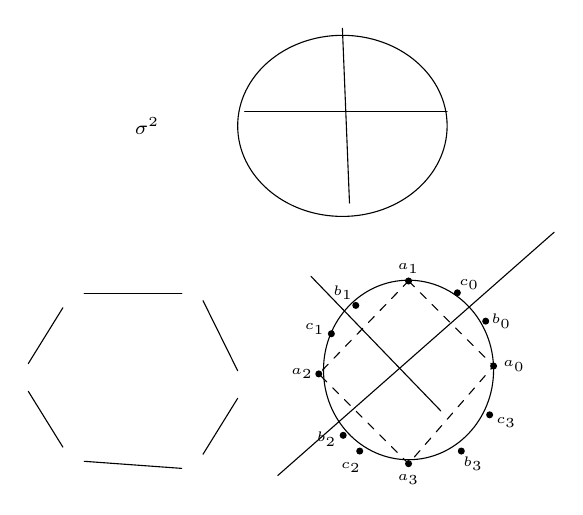
\begin{tikzpicture}[x=1mm,y=1mm,line cap=round,line join=round,font=\scriptsize]
\draw (61.7,-19.5) ellipse[x radius=13.3, y radius=11.5];
\draw (49.3,-17.7) -- (75,-17.7);
\draw (61.7,-7.1) -- (62.6,-29.3);
\node[inner sep=1pt] at (36.9,-19.5) {\scriptsize $\sigma^2$};
\draw (28.9,-40.8) -- (41.3,-40.8);
\draw (44,-41.7) -- (48.4,-50.6);
\draw (48.4,-54.1) -- (44,-61.2);
\draw (41.3,-63) -- (28.9,-62.1);
\draw (26.2,-60.3) -- (21.8,-53.2);
\draw (21.8,-49.7) -- (26.2,-42.6);
\draw (70.1,-50.5) ellipse[x radius=10.8, y radius=11.4];
\node[pt] at (70.1,-39.2) {};
\node[pt] at (76.3,-40.7) {};
\node[pt] at (79.9,-44.3) {};
\node[pt] at (80.9,-50) {};
\node[pt] at (80.4,-56.2) {};
\node[pt] at (76.8,-60.8) {};
\node[pt] at (70.1,-62.4) {};
\node[pt] at (63.9,-60.8) {};
\node[pt] at (61.8,-58.8) {};
\node[pt] at (58.7,-51) {};
\node[pt] at (60.3,-45.9) {};
\node[pt] at (63.4,-42.3) {};
\node[inner sep=1pt] at (70.1,-37.6) {\tiny $a_1$};
\node[inner sep=1pt] at (77.8,-39.7) {\tiny $c_0$};
\node[inner sep=1pt] at (81.9,-44.3) {\tiny $b_0$};
\node[inner sep=1pt] at (83.5,-50) {\tiny $a_0$};
\node[inner sep=1pt] at (82.5,-57.2) {\tiny $c_3$};
\node[inner sep=1pt] at (78.3,-62.4) {\tiny $b_3$};
\node[inner sep=1pt] at (70.1,-64.4) {\tiny $a_3$};
\node[inner sep=1pt] at (62.8,-62.9) {\tiny $c_2$};
\node[inner sep=1pt] at (59.7,-59.3) {\tiny $b_2$};
\node[inner sep=1pt] at (56.6,-51) {\tiny $a_2$};
\node[inner sep=1pt] at (58.2,-45.3) {\tiny $c_1$};
\node[inner sep=1pt] at (61.8,-40.7) {\tiny $b_1$};
\draw (57.7,-38.6) -- (74.2,-55.7);
\draw (53.5,-63.9) -- (88.6,-33);
\draw[dashed] (70.1,-39.2) -- (80.9,-50) -- (70.1,-62.4) -- (58.7,-51) -- cycle;
\end{tikzpicture}
\end{document}
